\chapter{Schedule}

\qquad At the start of the project a dedicated group meeting was performed in order to agree on a common project sequence, tasks and challenges as well as work distribution. This group meeting was deemed essential to structure the work packages and to achieve a consolidated baseline for the whole project including time line.\\

The result is a complex MS project Gantt diagram, which can be found in Annex 1.\\
\section{Initial Schedule}
\qquad The first version of the schedule starts with a project Kick-Off in October which is afterwards followed by a short planning phase. In this planning phase issues as scheduling, work distribution and scope of the project were addressed.\\

Subsequently, the definition phase started. Within this phase, the vehicle requirements were defined and the mission was planned, calculated and visualized in MATLAB. The outcomes of the definition phase are the boundary requirements which are set to provide a frame for both: the vehicle itself as well as the propulsion system. The requirements were defined at the beginning of the project and were verified after project completion.\\

Upon definition of the boundary requirements, the specification phase started. Within this phase, different propellant combinations were identified, discussed and compared. Additionally a first mass budget was calculated. The result of this phase is the system specification.\\

The sequence of the project includes several presentations. The first one was performed in October for a quick overview on the project planning. The second one after the boundary requirements and system specification was set. 
After this presentation, the vehicle and sub system design phase started. This phase included major parts of the work packages including propulsion system design with all sub-assemblies as RACS/ACS, propellant tanks, feeding and pressurization system, turbo pumps, catalyzer, engine, injector and nozzle. The outcome of this phase is a preliminary vehicle design and sub system design which was presented in the mid-term presentation.\\

As a last major work package the simulation phase started. The whole system was simulated including all sub systems and additionally the complex H2O2 decomposition regulation. The final presentation was performed after all tasks were completed and the simulation was finalized.\\

An overview the compressed initial schedule is shown in \autoref{Fig1}. The detailed Gantt schedule can be found in Annex 1.

\begin{figure}[H]
	\centering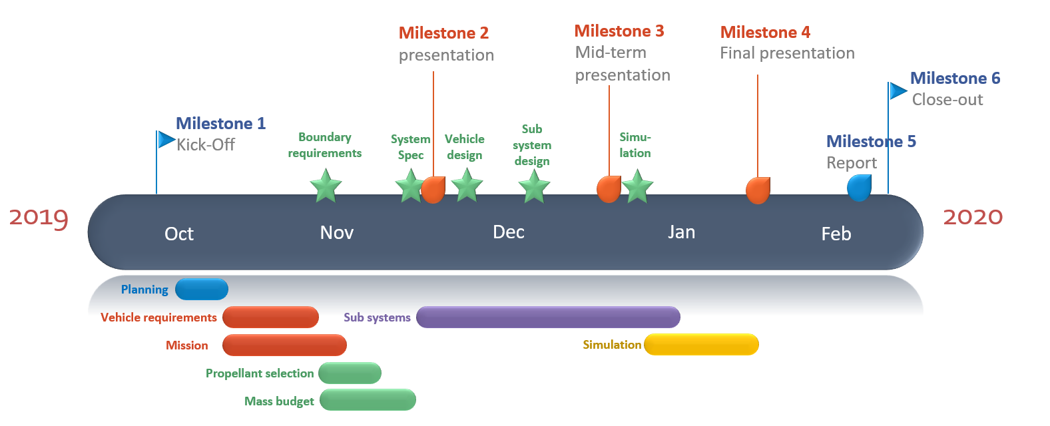
\includegraphics[width=\linewidth]{initialschedule}
	\caption{Initial schedule}\label{Fig1}
\end{figure}

\section{Final schedule – comparison as planned and as achieved}

\qquad As usual in project management and project work, not all milestones were achieved in time. As it is shown in the compressed final schedule in \autoref{Fig2}, the finalized vehicle design, the finalized sub system design and the corresponding simulation shifted within the project schedule (\autoref{Fig2}, shown in red). Nevertheless all work packages have been successfully completed until Milestone 4, the final presentation.

\begin{figure}[H]
	\centering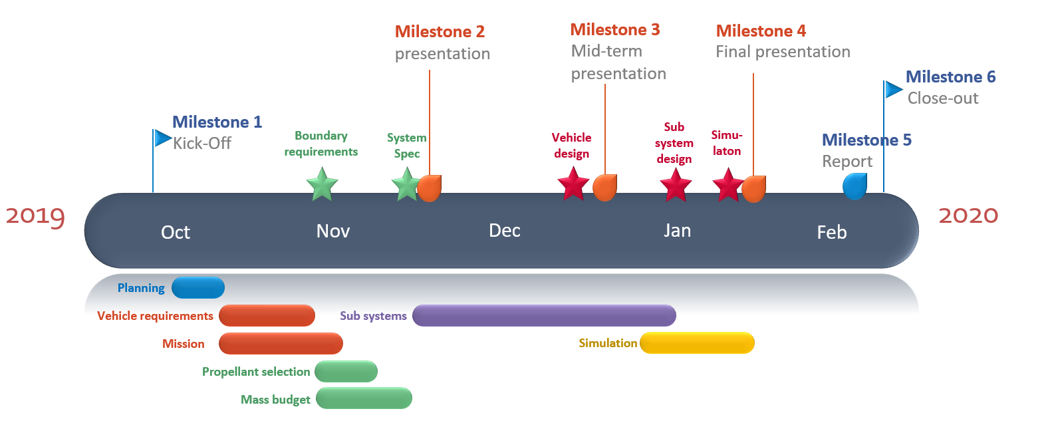
\includegraphics[width=\linewidth]{finalschedule}
	\caption{Final schedule - comparison as planned and as achieved}\label{Fig2}
\end{figure}

